\documentclass[diploma]{nanolab2015}

\begin{document}
\begin{titlepage}
\begin{center}
    \large
    ФЕДЕРАЛЬНОЕ ГОСУДАРСТВЕННОЕ БЮДЖЕТНОЕ ОБРАЗОВАТЕЛЬНОЕ УЧРЕЖДЕНИЕ ВЫСШЕГО ОБРАЗОВАНИЯ «МОСКОВСКИЙ ГОСУДАРСТВЕННЫЙ УНИВЕРСИТЕТ ИМЕНИ М.В.ЛОМОНОСОВА»
     
    \textbf{Физический факультет}\\
    \vspace{4cm}
    \textsc{\Large Отчет по практическому заданию №2 (13.3(6))}\\[5mm]
    {\LARGE Численные методы в физике.}
\end{center}
\vspace{7cm}
\null
\begin{flushright}
\normalsize студента 427 группы
\\Иванова Ивана Ивановича
\end{flushright}
\vfill
\begin{center}
\textbf{Москва - 2022}
\end{center}
\end{titlepage}

\section{Постановка задачи.}
Численно решить выписанную ниже задачу Коши  на отрезке $t= [0, 20]$ для $v_0= 0$ и $u_0 = \frac{401}{30}$,  используя двухслойную схему с перешагиваем (Leapfrog method).

\begin{equation*}
\begin{cases}
   \frac{d^2 u}{d t^2} + u = 0\\
   u(t=0)=u_0 = \frac{401}{30}\\
   \dot u(t=0)= v_0 =0
 \end{cases}
\end{equation*}

Необходимо рассмотреть три варианта шага интегрирования:

1) На границе устойчивости

2) Шаг в два раза меньше предыдущего

3) Шаг в 10 раз меньше шага на границе устойчивости

Также для расчета значений функций в следующем за начальным узлом сетки используется способа:

 1) один шаг по схеме Эйлера 
 
 2)схему Эйлера с шагом в 2 раза меньше шага основной сетки  
 
 3)схему Эйлера с шагом в 10 раз меньше шага основной сетки 

\section{Аналитическое решение.}
Общее решение данной задачи Коши известно и оно задаётся следующим выражением:

$$u(t) = A \cos(t) + B \sin(t)$$ 

Подставляя начальные условия в общее решение получаем точное (аналитическое) решение поставленной задачи Коши:
$$u(t) = \frac{401}{30} \cos(t)$$ 

 \section{Численное решение.}
Для численного решения представлю исходное уравнение второго порядка в виде системы двух уравнений первого порядка с помощью следующей замены: $\dot u =v$. Получим следующую систему уравнений:
 
 \begin{equation*}
\begin{cases}
    \frac{d v}{d t} = - u\\
    \frac{d u}{d t} =  v\\
   u(t=0)=u_0\\
   v(t=0)= v_0
 \end{cases}
\end{equation*}

Численно буду решать именно данную систему уравнений. Для целей аналитических оценок устойчивости и порядка аппроксимации численного метода данное уравнение также можно записать в следующем комплексном виде, где $U = u + i v$:

\begin{equation*}
\begin{cases}
   \frac{d U}{d t} = -i U = f(U,t)\\
   U(t=0)=u_0 + i v_0
 \end{cases}
\end{equation*}

Численное решение осуществляется с помощью двухслойного метода с перепрыгиванием (Leapfrog).

\section{Исследование двухслойного численного метода с перепрыгиванием.}
Выпишу явно схему данного численного метода.

$$U_{n+1} = U_{n-1} + f_{n} 2 \Delta t$$

Найду оценку погрешности данного метода, для этого рассмотрю некоторую функцию $U(t)$ непрерывных переменных. Разложу функции $U(t_{n \pm 1})$ в ряд Тейлора в точке $t_n$:

$$U_{n+1} = U_n + \frac{\partial U}{\partial t} \Delta t + \frac{1}{2} \frac{\partial^2 U}{\partial t^2} \Delta t^2 + \frac{1}{6} \frac{\partial^3 U}{\partial t^3} \Delta t^3$$

$$U_{n-1} = U_n - \frac{\partial U}{\partial t} \Delta t + \frac{1}{2} \frac{\partial^2 U}{\partial t^2} \Delta t^2 - \frac{1}{6} \frac{\partial^3 U}{\partial t^3} \Delta t^3$$

Подставляем эти выражения в исходную разностную схему и получаем:

$$\frac{\partial U}{\partial t} + \frac{1}{6} \frac{\partial^3 U}{\partial t^3} \Delta t^2 = f_n$$

Вычитая из этого выражения точный дифференциальный оператор получим оценку для ошибки данной схемы:

$$z_n = \frac{1}{6} \frac{\partial^3 U}{\partial t^3} \Delta t^2 = O(\Delta t^2)$$

Метод имеет второй порядок точности по $\Delta t$.

Теперь исследую устойчивость данного метода. Пусть $\epsilon_n$ - ошибка решения на n-ом шаге, тогда запишем уравнение:

$$U_{n+1} +  \epsilon_{n+1}= U_{n-1} +   \epsilon_{n-1}+ f_{n}(U_n +   \epsilon_n) 2 \Delta t$$

Разложу функцию f по U и подставлю уравнению. Тогда получим следующее уравнение для ошибки $\epsilon$:

$$\epsilon_{n+1} = \epsilon_{n-1} + \frac{\partial f}{\partial U} \epsilon_n 2 \Delta t$$

Введу множитель перехода $\lambda$, такой, что $\epsilon_{n+1}=\lambda \epsilon_n$, тогда получим следующее квадратное уравнение на поиск $\lambda$:

$$\lambda^2 - 2 \frac{\partial f}{\partial U} \Delta t \lambda - 1 = 0$$

Решение уравнения имеет следующий вид: 

$$\lambda_{1,2} = \frac{\partial f}{\partial U} \Delta t \pm \sqrt{ \frac{\partial f}{(\partial U} \Delta t)^2+1}$$

Теперь рассмотрим конкретно нашу задачу: осцилляторное решение, где $f(U,t) = -i \omega U$, где $\omega$ -  собственная частота осциллятора, тогда:

$$\lambda_{1,2} = -i \omega \Delta t \pm \sqrt{1-(\omega \Delta t)^2}$$

Если $ \omega \Delta t \leq 1$, то  $|\lambda_{1,2} | \leq 1$, схема является условно устойчивой.

Условие устойчивости: $\Delta t	\leq \frac{1}{\omega}$. В конкретно нашей задаче частота равна 1, а значит, что шаг  $\Delta t$ должен быть меньше 1.

При этих условиях двухслойная схема с перешагиваем (Leapfrog method) устойчива и сходится к аналитическому решению со вторым порядком по времени.

\section{Результаты численного решения.}

Языком для реализации численного метода выбран Python и библиотеки numpy и matplotlib.

Особенность моей реализации численного метода для этой задачи заключается в том, что  не смотря на то, что в правой части нет явной зависимости от времени, время всё равно вычисляется и передаётся во все функции, т.е. данный алгоритм может решать задачи, у которых правая часть уравнения явно зависит от времени без модификаций в алгоритме. Также стоит отметить, что при минимальных изменениях в коде, данный алгоритм способен решать систему из n дифференциальных уравнений первого порядка благодаря векторной записи вычислений. Все графики были построены внутри самой программы.

На графиках ниже представлены численные решения при различных шагах по времени. Видно, что если брать $\Delta t = 1$, то даже качественное решение получить невозможно. Также видно, что при таком шаге решение расходится. Если же взять шаг в 2 раза меньше, то уже можно получить решение, качественно напоминающее косинус, также стоит отметить, что решение не расходится. Если же шаг уменьшить в 10 раз, то уже получаем очень хорошее соответствие с точным решением.  

При же увеличении количества шагов в схеме Эйлера уменьшается "начальная" ошибка метода Leapfrog.

Видно, что ошибка численного решения осциллирует и чем меньше шаг, тем меньше максимальное значение ошибки соответственно. Так же видно, что максимальное значение ошибки при каждом шаге растёт с увеличением t.

1) Метод Эйлера имеет первый порядок аппроксимации по времени, двухслойный метод с перепрыгиванием имеет второй порядок точности, поэтому, чтобы не "ухудшать" порядок аппроксимации Leapfrog необходимо выбирать шаг схемы Эйлера, равной квадрату шага схемы с перепрыгиванием. В самой же работе видна зависимость погрешности решения от точности первого шага по схеме Эйлера.

2) Условие устойчивости имеет вид: $\Delta t \leq \frac{1}{\omega}$, однако в работе было продемонстрировано, что значение шага, взятое на границе устойчивости даёт только качественное поведение решения. Тоже самое можно сказать про шаг в два раза меньший, чем $\frac{1}{\omega}$. Хорошая точность получена на шаге в 10 раз меньшим, чем $\frac{1}{\omega}$. Я бы назвал это значение оптимальным по временным затратам и полученной точности решения. Если же необходимо рассматривать поведение решения на временах больших, нежели рассмотренных в данной задаче 20 секунд, то шаг сетки стоит уменьшить.

3) Также стоит отметить, что собственная частота может быть довольно маленькой величиной, как и рассматриваемый промежуток времени, из-за чего решение может выглядеть "угловатым" из-за большого шага по сравнению с интервалом времени. В таком случае можно уменьшить шаг, если это позволяют вычислительные ресурсы, в эстетических целях.

\begin{figure}[h!]
\centering
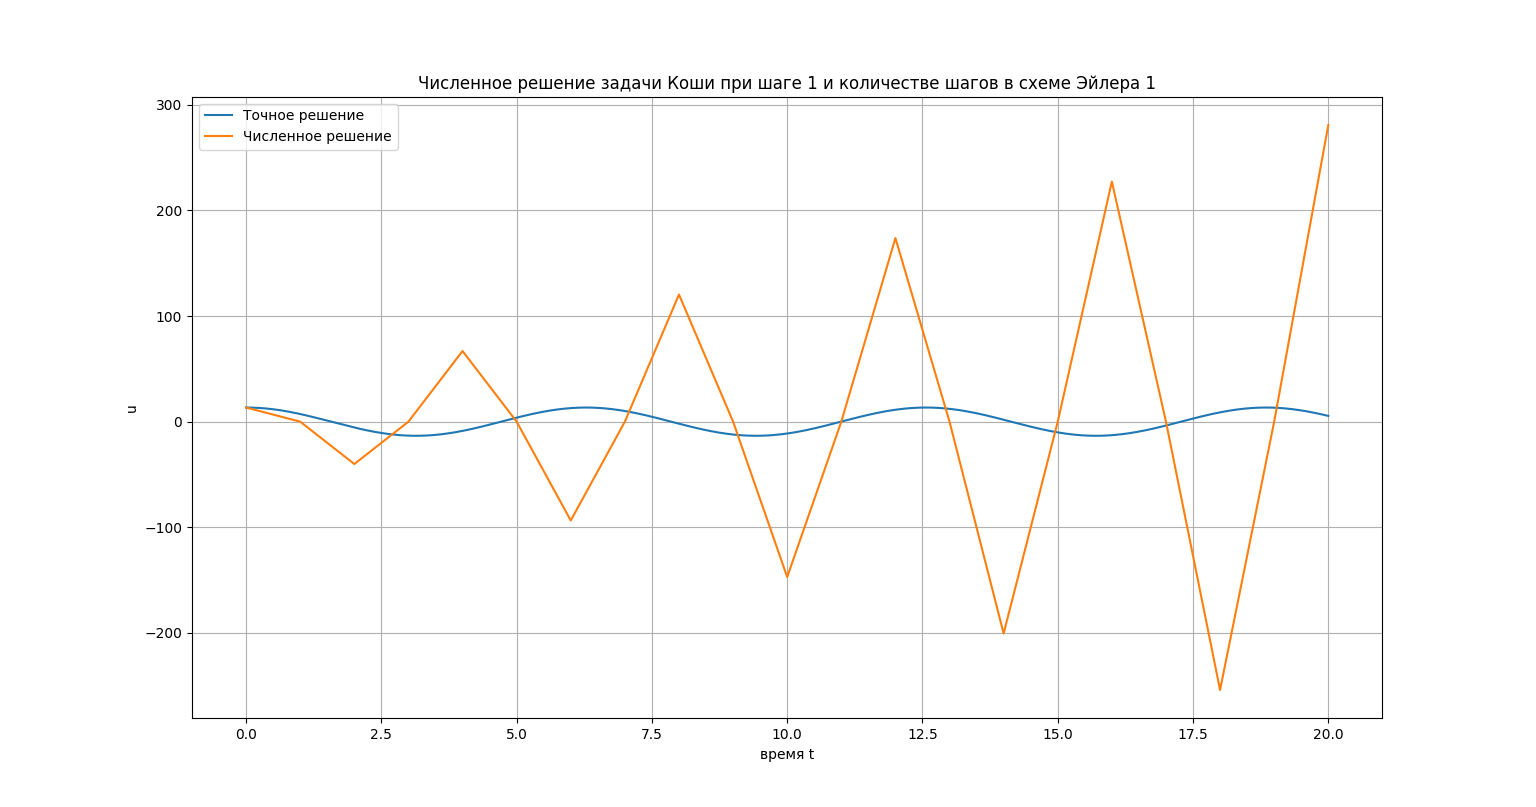
\includegraphics[scale=0.5]{1 1.png}
\end{figure}

\begin{figure}[h!]
\centering
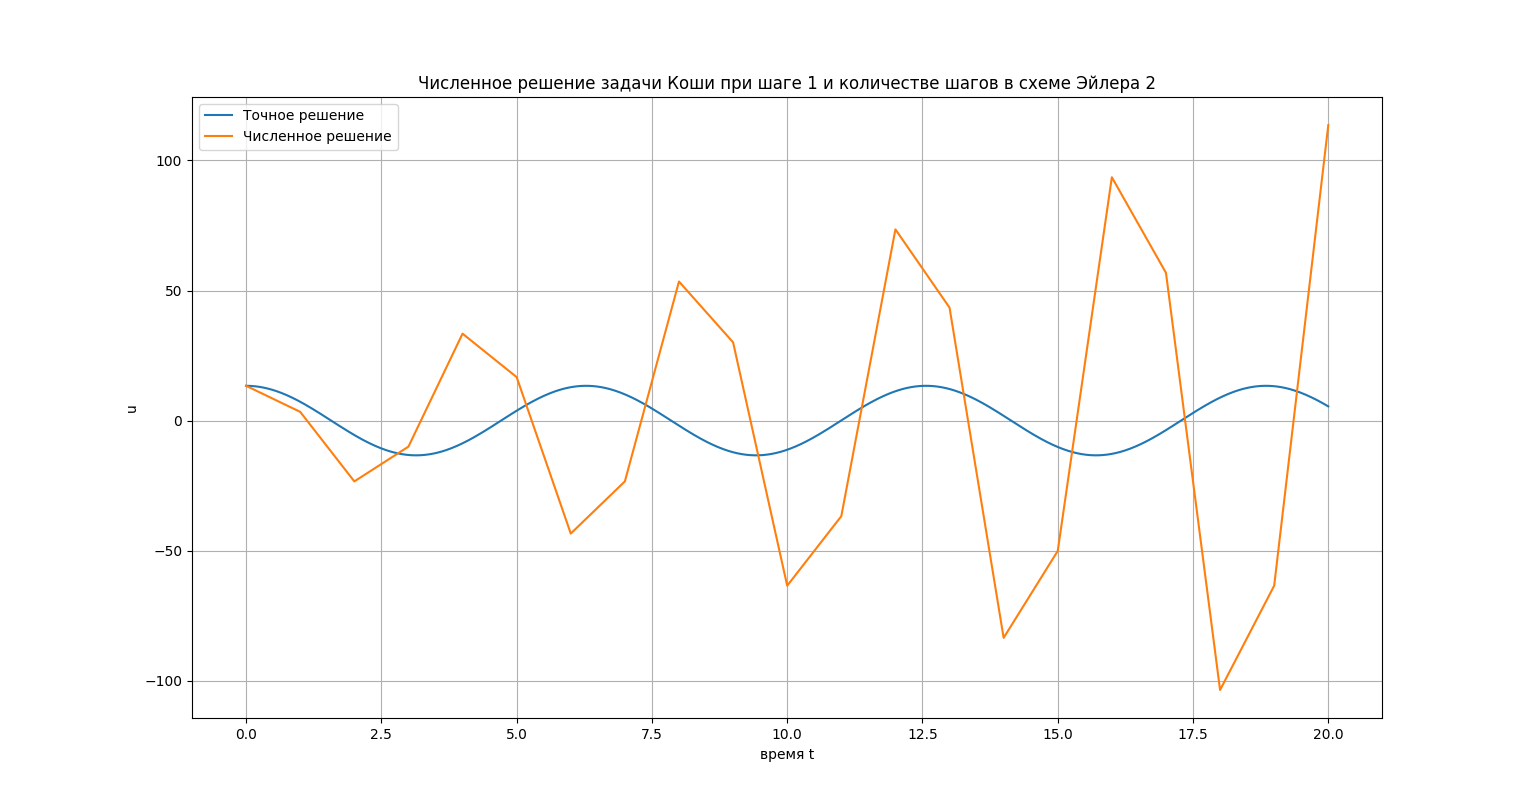
\includegraphics[scale=0.5]{1 2.png}
\end{figure}

\begin{figure}[h!]
\centering
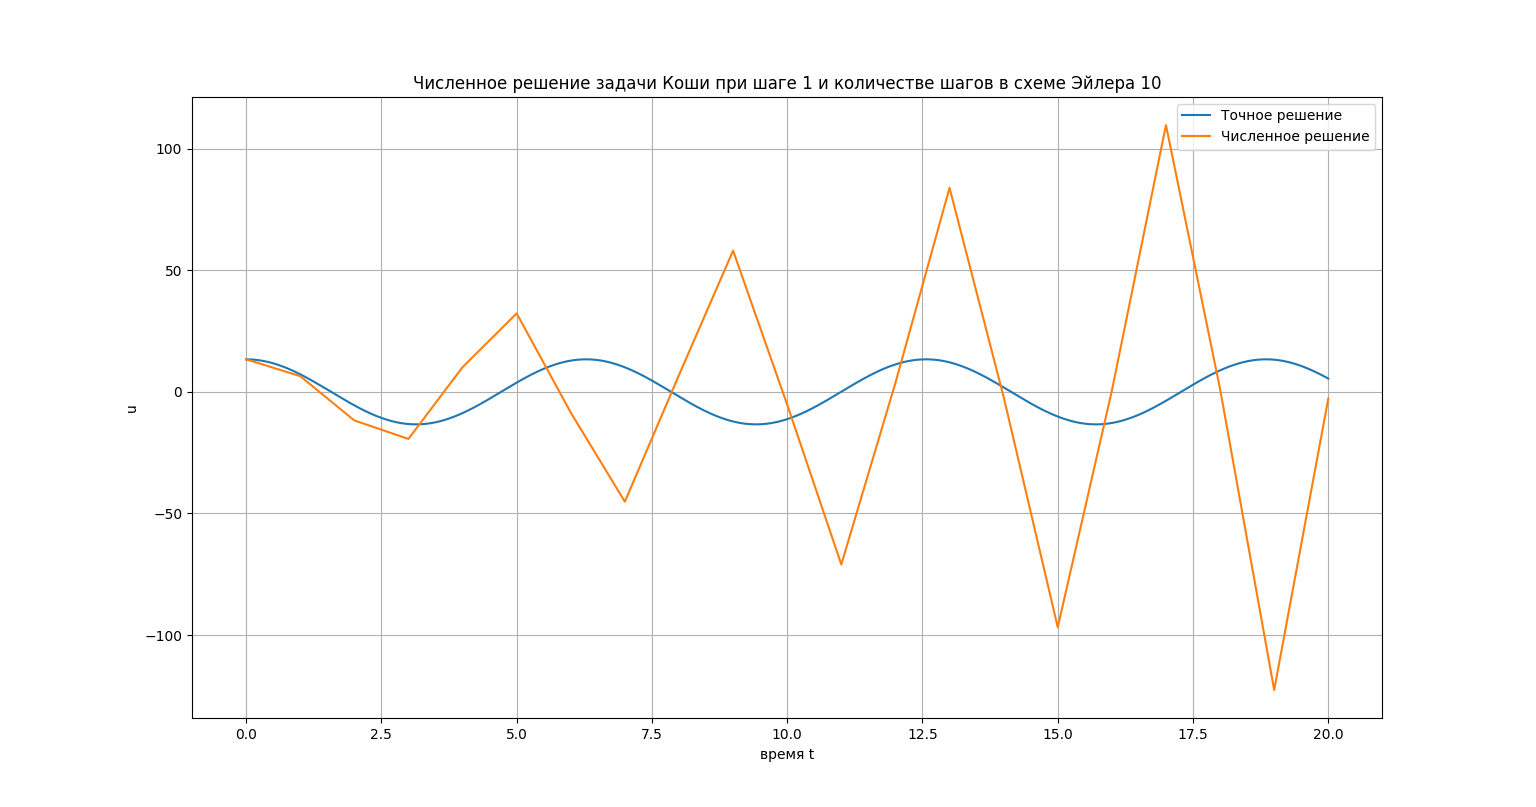
\includegraphics[scale=0.5]{1 10.png}
\end{figure}

\begin{figure}[h!]
\centering
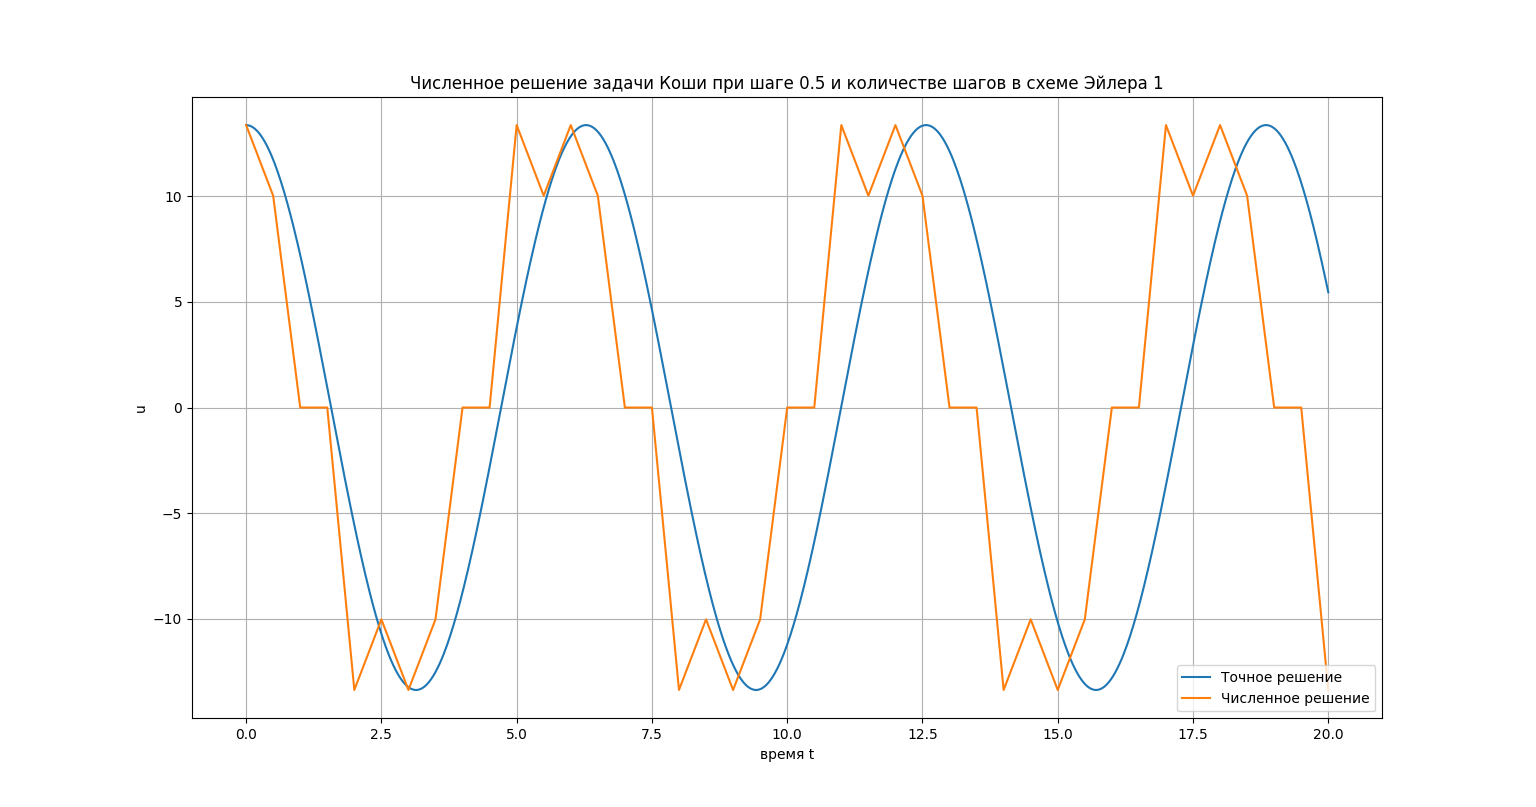
\includegraphics[scale=0.5]{05 1.png}
\end{figure}

\begin{figure}[h!]
\centering
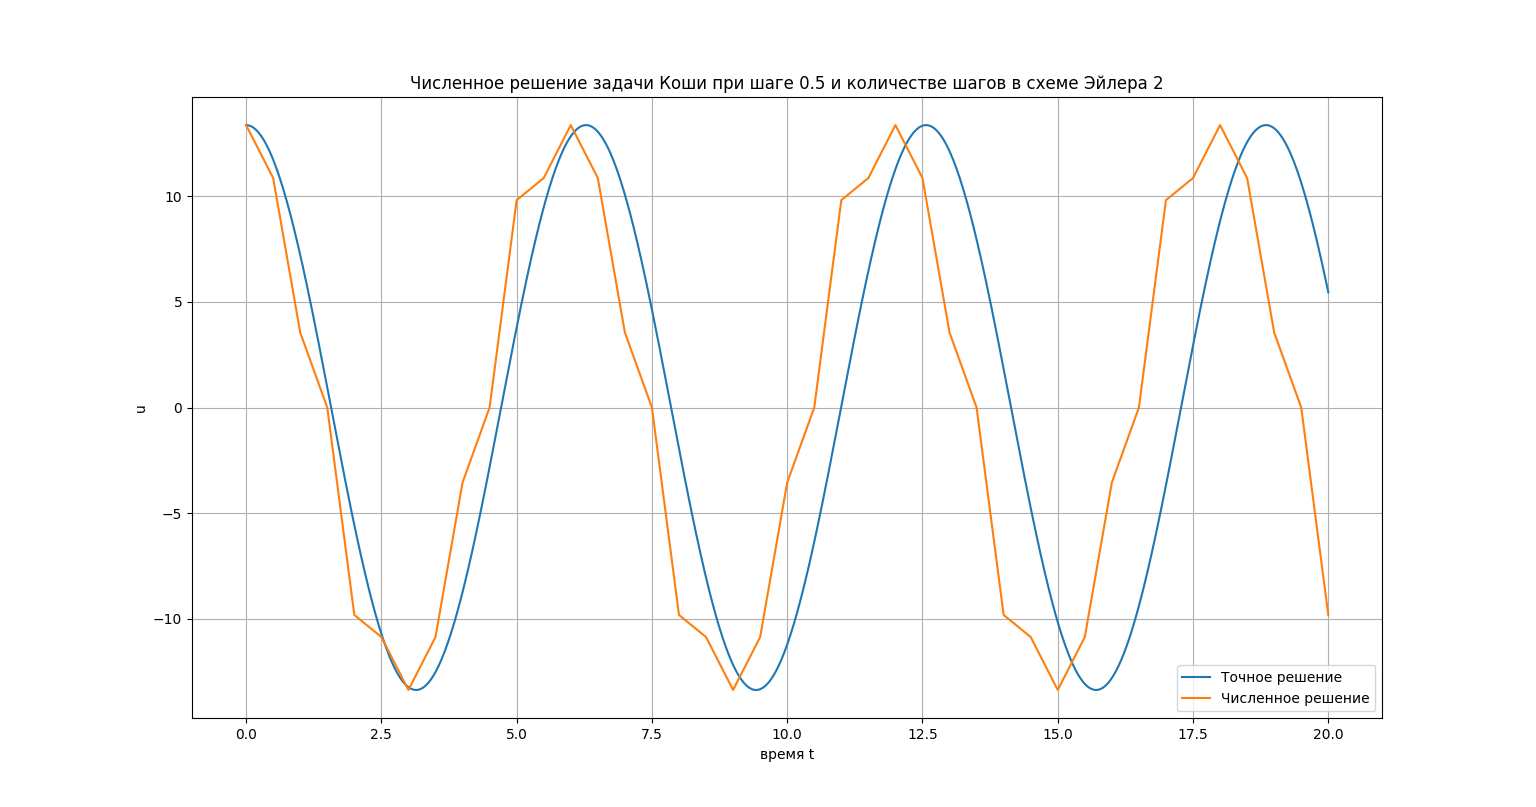
\includegraphics[scale=0.5]{05 2.png}
\end{figure}

\begin{figure}[h!]
\centering
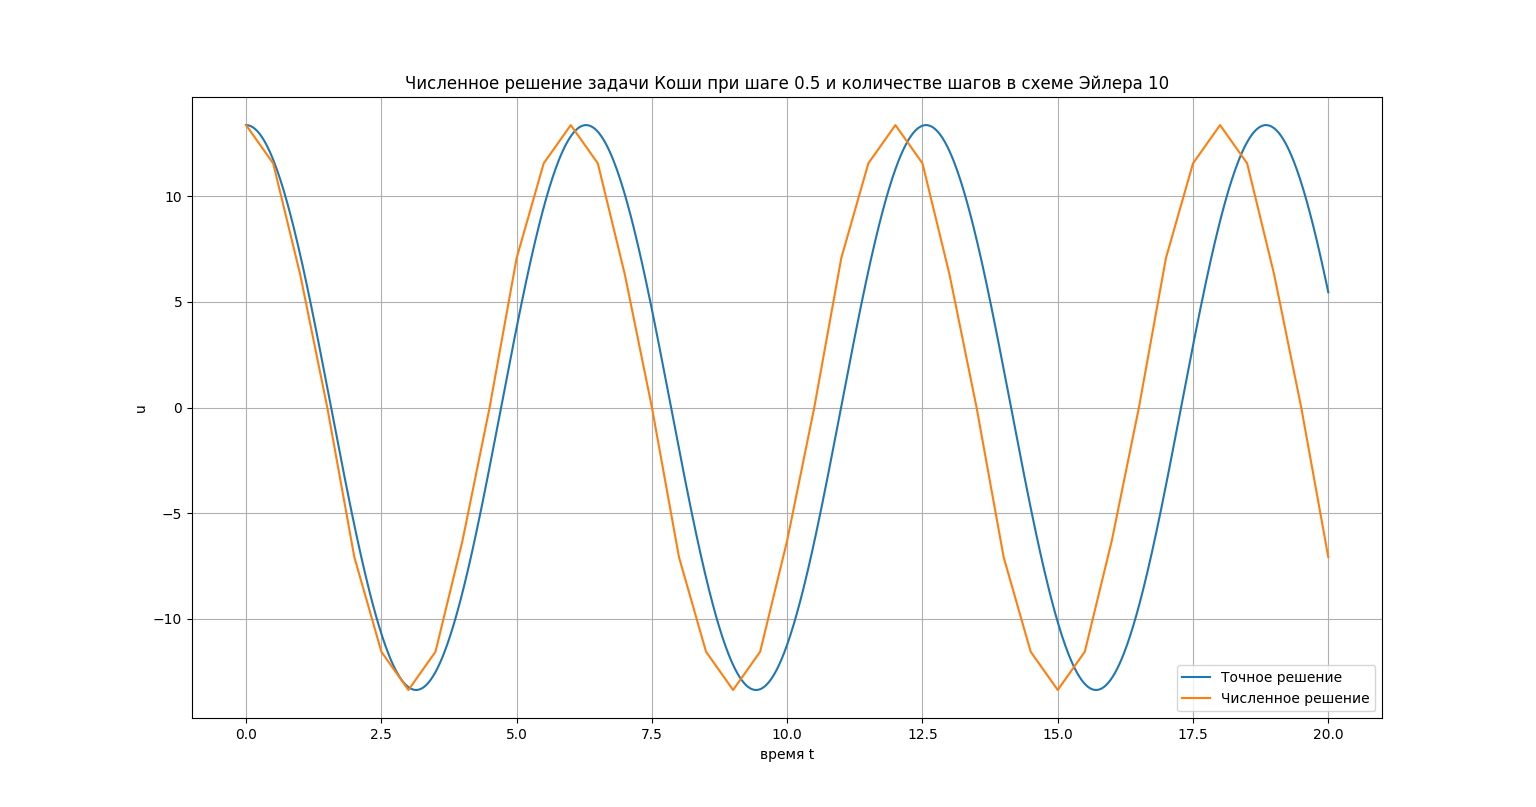
\includegraphics[scale=0.5]{05 10.png}
\end{figure}

\begin{figure}[h!]
\centering
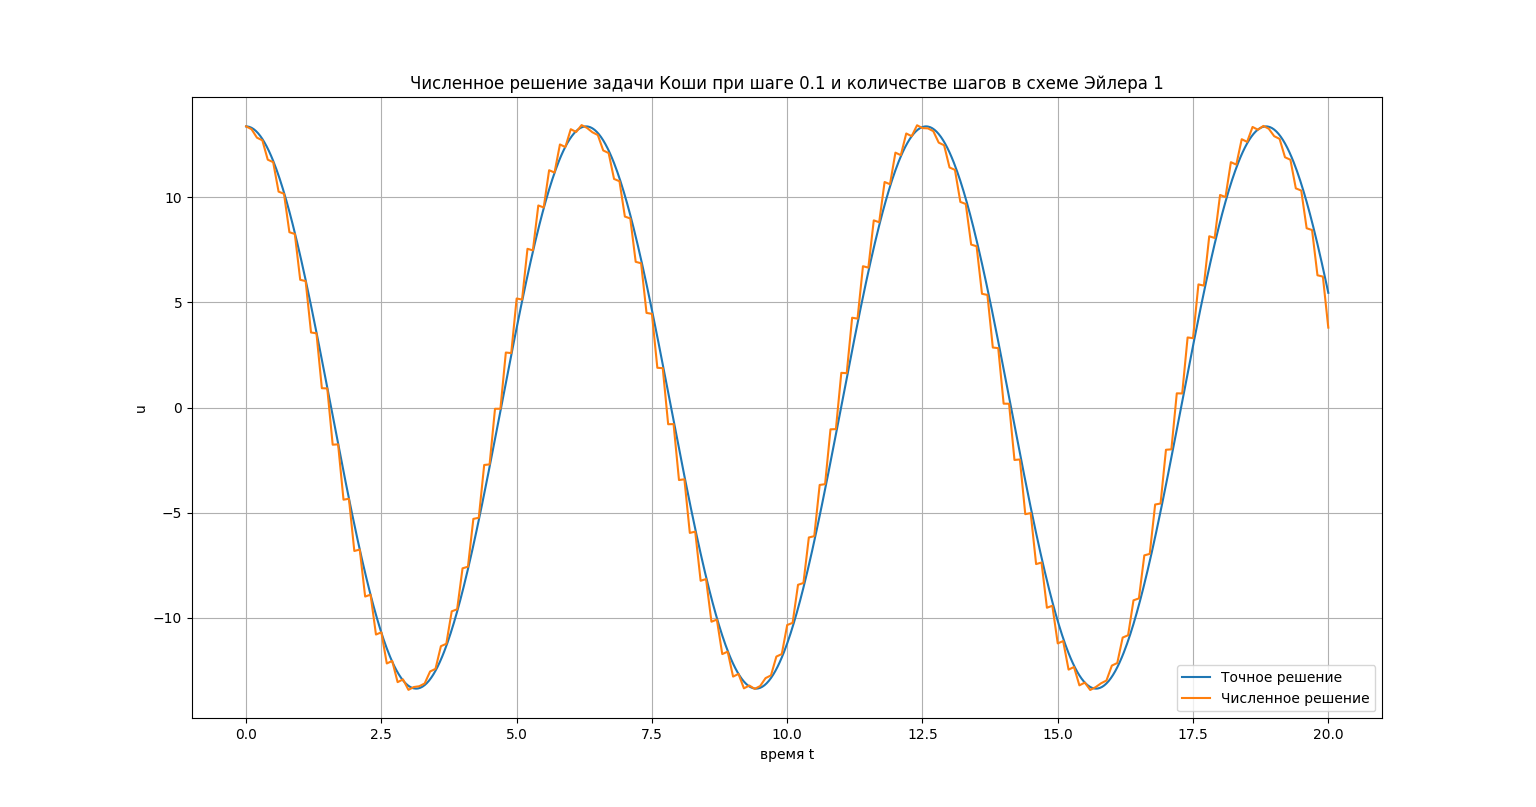
\includegraphics[scale=0.5]{01 1.png}
\end{figure}

\begin{figure}[h!]
\centering
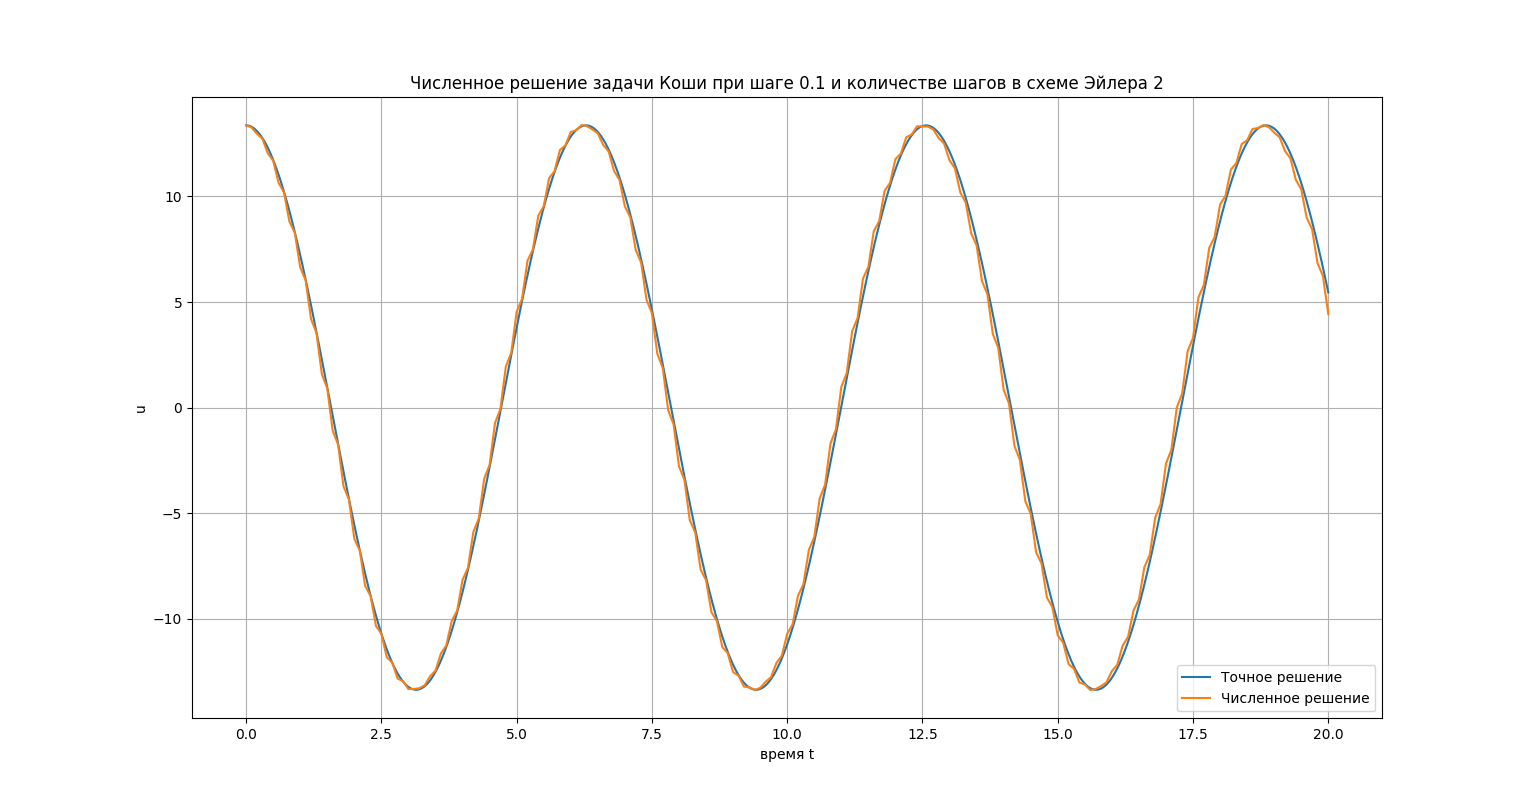
\includegraphics[scale=0.5]{01 2.png}
\end{figure}

\begin{figure}[h!]
\centering
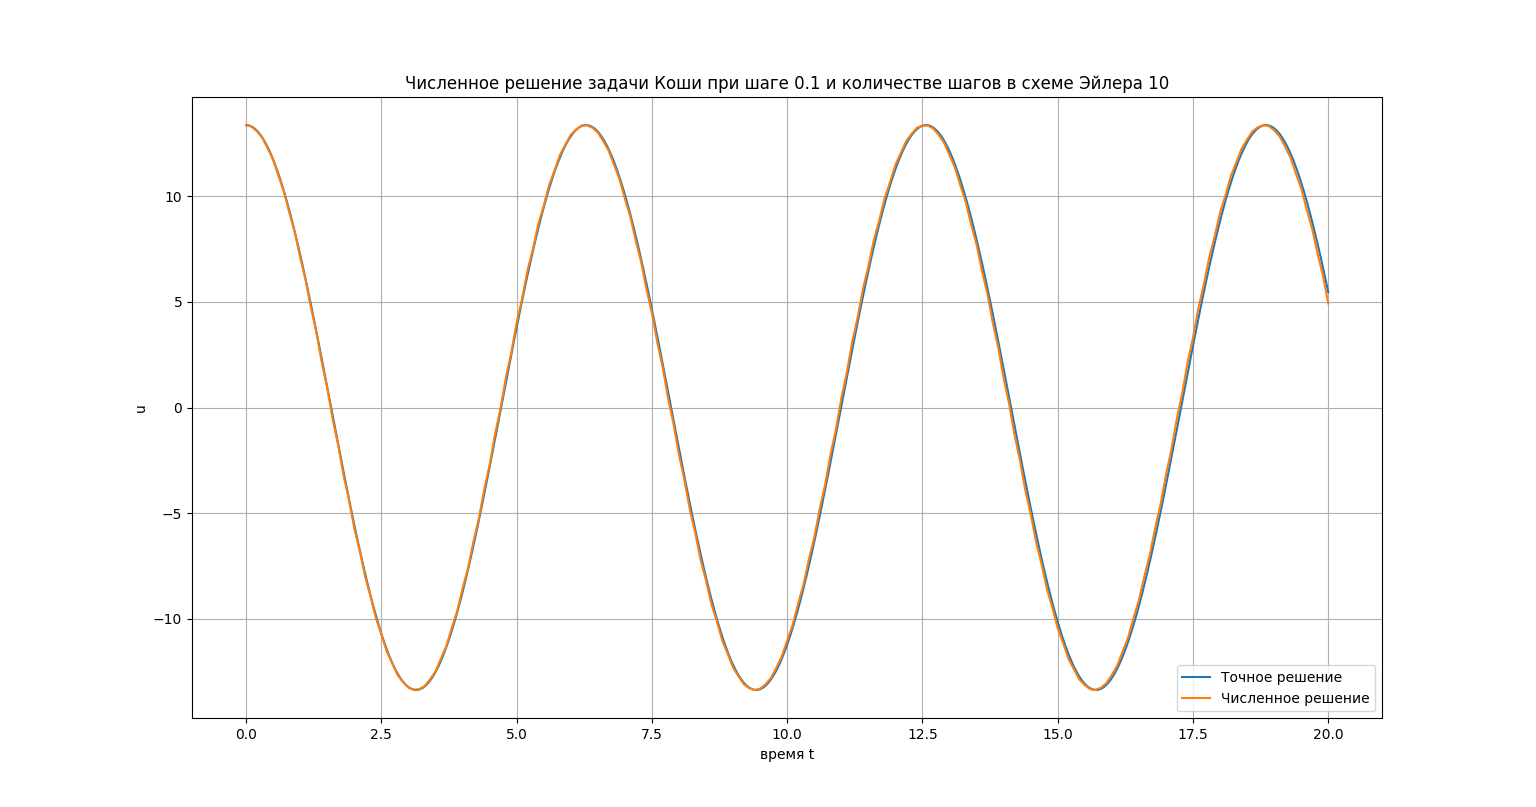
\includegraphics[scale=0.5]{01 10.png}
\end{figure}

\begin{figure}[h!]
\centering
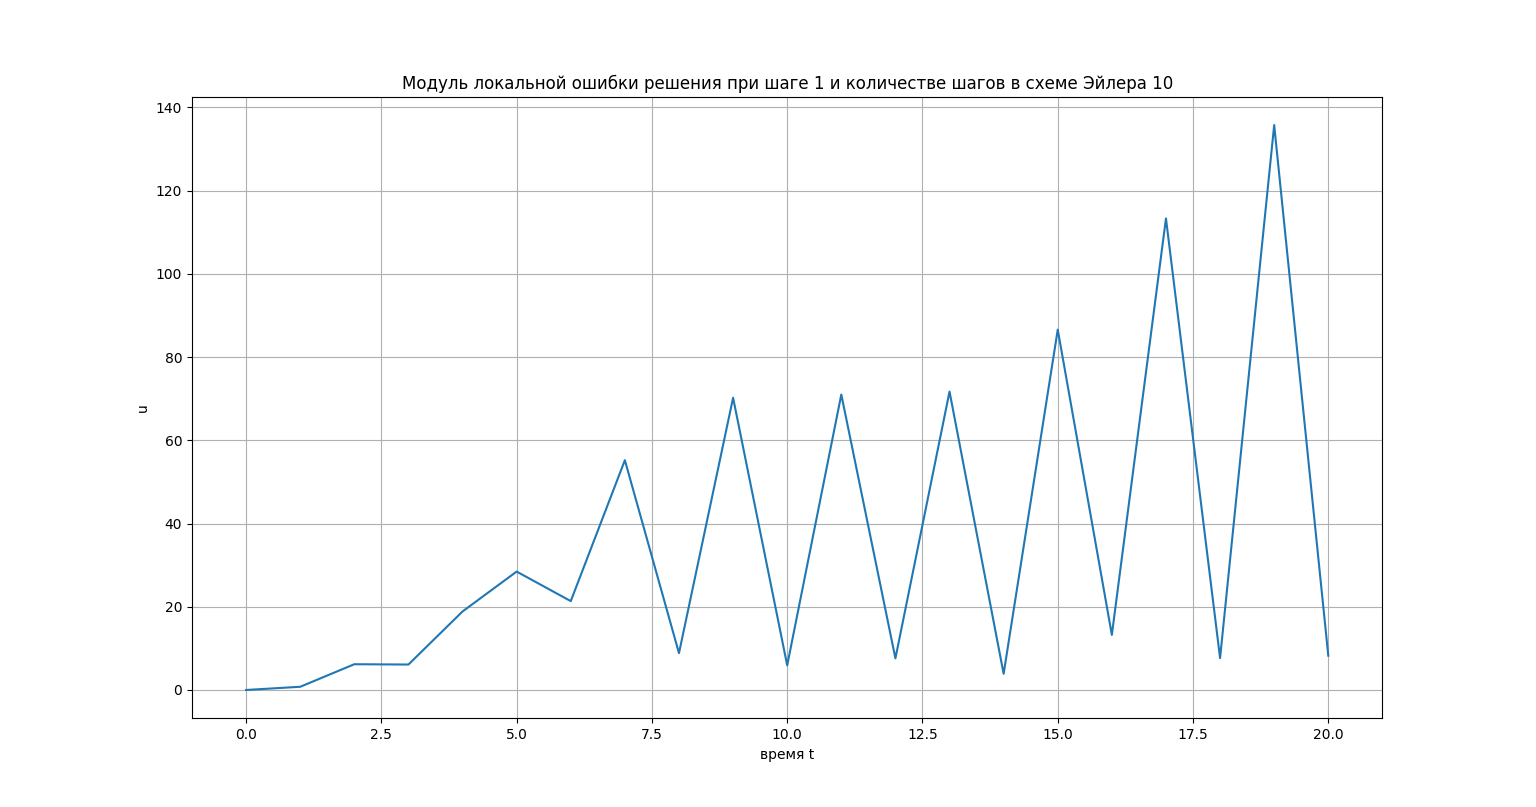
\includegraphics[scale=0.5]{err 1.png}
\end{figure}

\begin{figure}[h!]
\centering
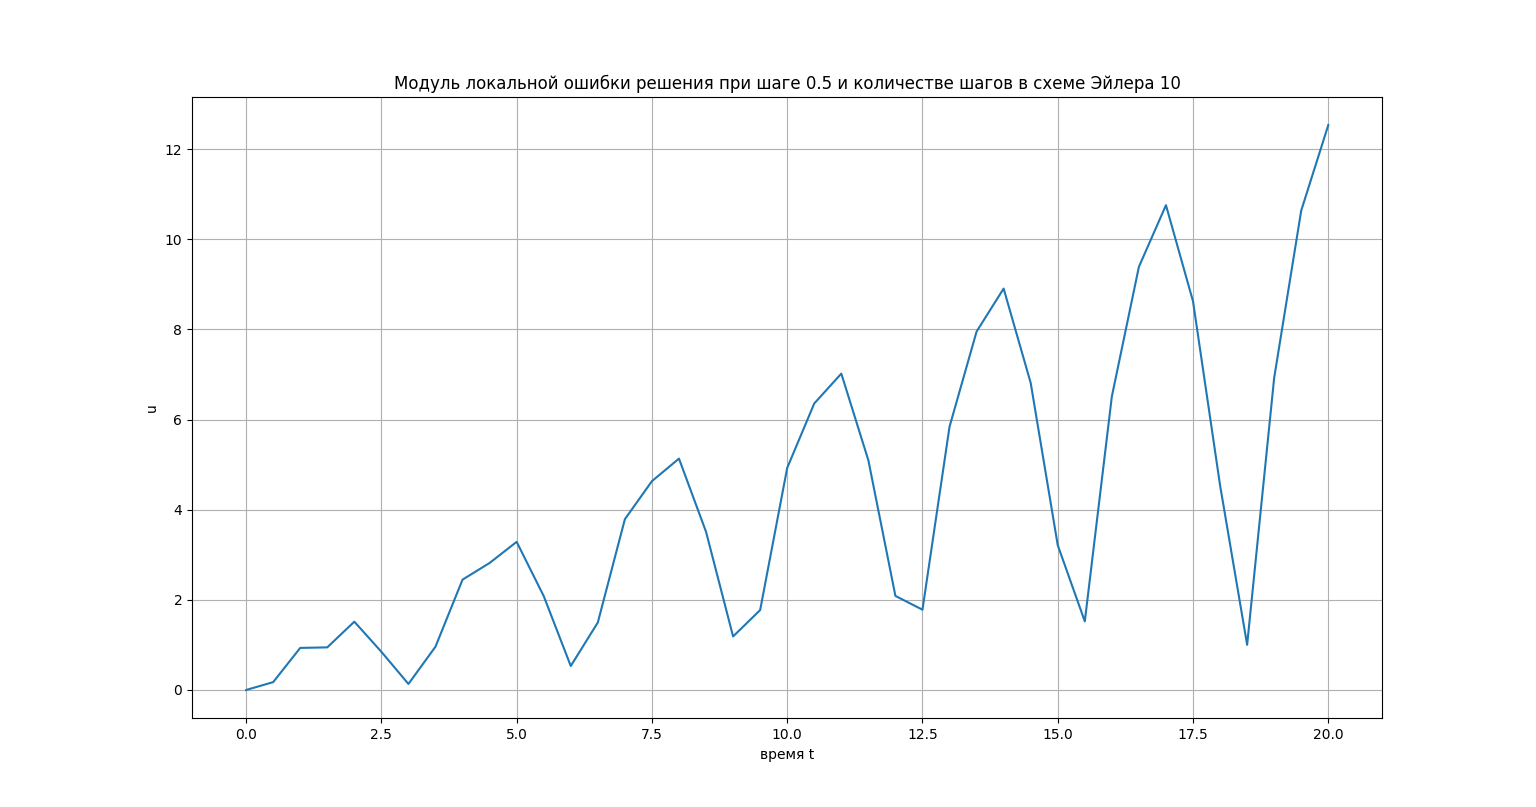
\includegraphics[scale=0.5]{err 05.png}
\end{figure}

\begin{figure}[h!]
\centering
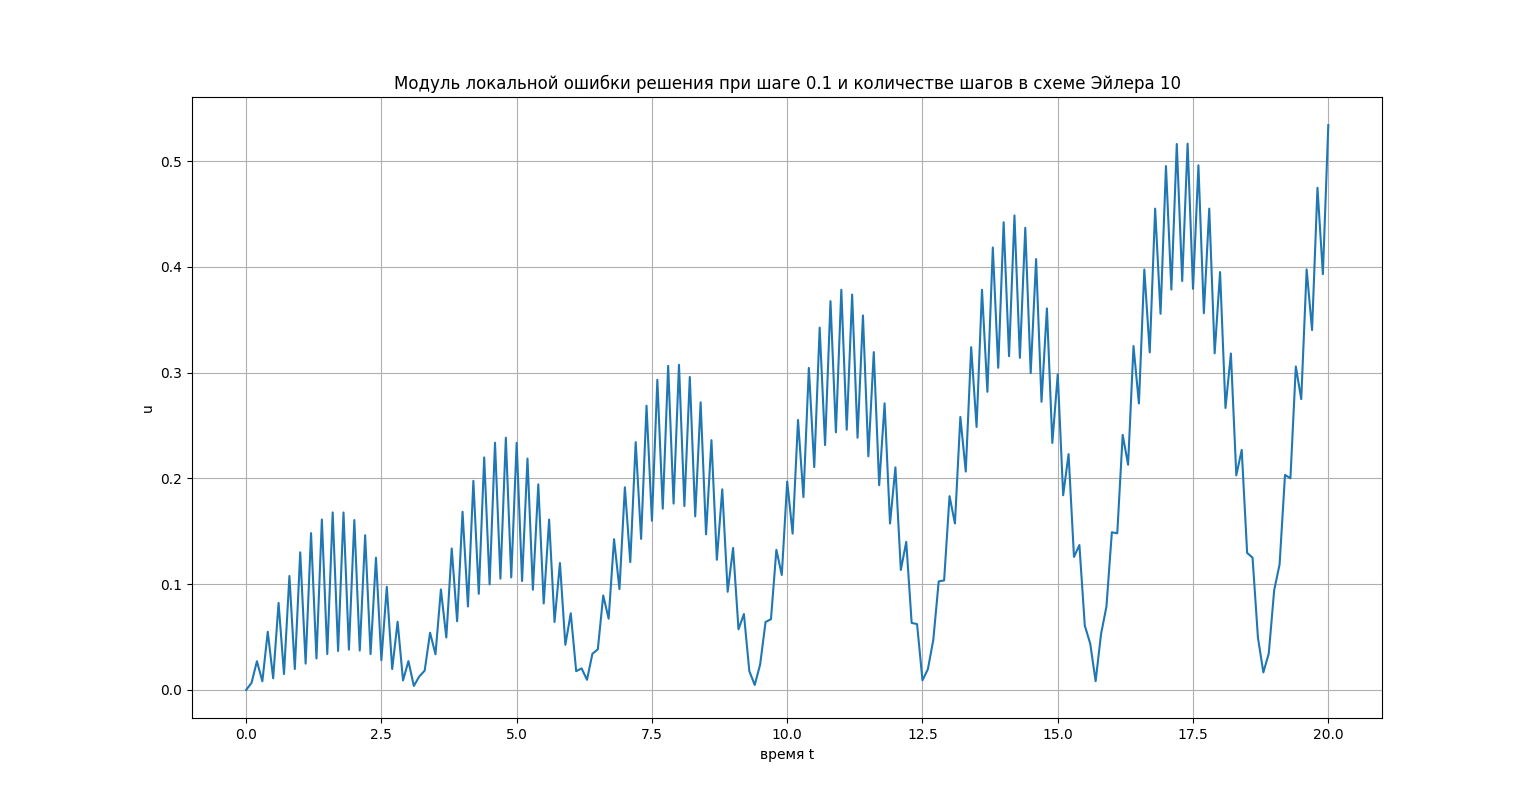
\includegraphics[scale=0.5]{err 01.png}
\end{figure}

\begin{figure}[h!]
\centering
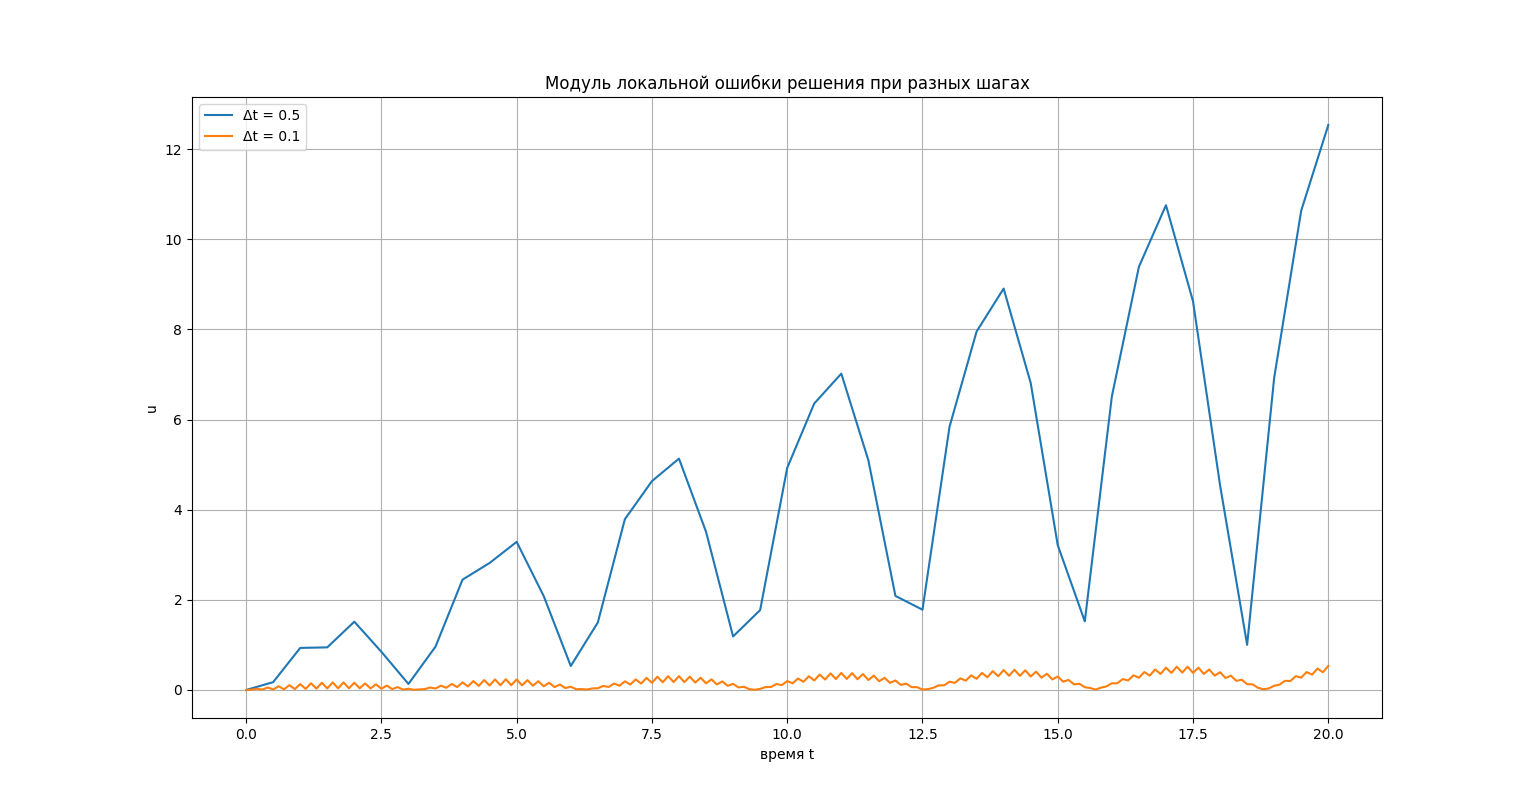
\includegraphics[scale=0.5]{err t.png}
\end{figure}

\end{document}